\documentclass{standalone}
\usepackage{tikz}
\usetikzlibrary{shapes}
\usepackage{arydshln}
\begin{document}
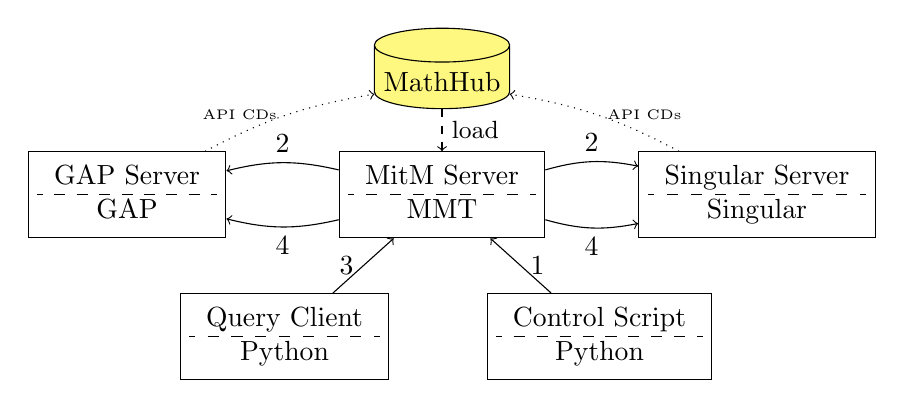
\begin{tikzpicture}[xscale=2, yscale=1.8]\normalsize
   \tikzstyle{database} = [cylinder,cylinder uses custom fill,
      cylinder body fill=yellow!50,cylinder end fill=yellow!50,
      shape border rotate=90, 
      aspect=0.25,draw]
  \node[draw] (g) at (0,0) {
    \begin{tabular}{c}
      GAP Server \\\hdashline GAP
    \end{tabular}
  };
  \node[draw,database] (mh) at (2,.8) {MathHub};
  \node[draw] (m) at (2,0) {
    \begin{tabular}{c}
      MitM Server\\\hdashline MMT
    \end{tabular}
  };
  \node[draw] (s) at (4,0) {
    \begin{tabular}{c}
      Singular Server\\\hdashline Singular
    \end{tabular}
  };
  \node[draw] (p) at (1, -1) {
    \begin{tabular}{c}
      Query Client\\\hdashline Python
    \end{tabular}
  };
  \node[draw] (c) at (3, -1) {
    \begin{tabular}{c}
      Control Script\\\hdashline Python
    \end{tabular}
    };
    \draw[dashed,->] (mh) -- node[right] {\small load} (m);
    \draw[dotted,->] (g) to[bend left=10] node[left] {\tiny API CDs} (mh); 
    \draw[dotted,->] (s) to[bend right=10]  node[right] {\tiny API CDs} (mh); 
    \draw[->] (c) to node[right] {1} (m);
    \draw[->] (m) to[bend left=15] node[above] {2} (s);
    \draw[->] (m) to[bend right=15] node[above] {2} (g);
    \draw[->] (p) to node[left] {3} (m);
    \draw[->] (m) to[bend right=15] node[below] {4} (s);
    \draw[->] (m) to[bend left=15] node[below] {4} (g);
  \end{tikzpicture}
\end{document}
% LocalWords:  tikzpicture xscale yscale Singuler

%%% Local Variables:
%%% mode: latex
%%% TeX-master: t
%%% End:
